\documentclass[a4paper, 14pt]{extarticle}

\usepackage{../generalPreamble}
\usepackage{../conspectFormat}

\begin{document}
\begin{titlepage}
    {\centering
        {\bfseries
            
\includegraphics[height=8cm]{../res/logo.jpeg}\\
            Unity. Precision. Perfection.\\
            \vspace{3.5cm}
            \uppercase{Конспект лекций} \\
            по дисциплине \enquote{Безопасность жизнедеятельности}\\
        }
        \vspace{\fill}
    }
    \begin{tabular}{l l}
        \textbf{Лектор}: & Трусов Александр Олегович\\
        \textbf{Страниц}: &\pageref{LastPage}\\
        \textbf{Последнее обновление}: & \today{}\\ 
        \textbf{Автор}: & Корытов Павел, 6304\\
    \end{tabular}

    \vspace{2cm}
    {\centering
        Санкт-Петербург \\
        \the\year\\
    }
\end{titlepage}

\tableofcontents
\newpage

\section{Введение}
\dfn{Опасность} --- совокупность явлений, процессов, объектов, способных в определённых условиях наносить ущерб здоровью человека непосредственно или косвенно, т.е. вызывать нежелательные последствия (события)

Виды опасности:
\begin{itemize}
    \item Реальная
    \item Потенциальная или скрытая
\end{itemize}

Влияние на человека:
\begin{itemize}
    \item Прямое
    \item Косвенное
\end{itemize}

\subsubsection*{Аксиомы БЖД}
\begin{enumerate}
    \item Любая человеческая деятельность потенциально опасна
    \item С развитием техники опасность увеличивается
\end{enumerate}

\subsubsection*{Классификация опасностей}
\begin{itemize}
    \item По природе происхождения
    \item По эффекту воздействия
    \item По вызываемым последствиям
    \item По приносимому ущербу
    \item По сфере проявления опасностей
\end{itemize}

\dfn{Опасный фактор (ОПФ)} --- воздействие на работающего, которое в ограниченное время может привести к травме или другому внезапному резкомму ухудшению здоровья

\dfn{Вредный фактор (ВПФ)} --- воздействие на работающего, которое в определённых условия в течение длительного времени ведет к заболеванию или ухудшению здоровья

\subsection{Теория риска}
Абсолютная безопасность, как правило, технически недостижима

\dfn{Риск} (степень риска, уровень риска) --- это частота реализации опасности
\begin{equation}
    R = nN,
\end{equation}
где:
\begin{itemize}
    \item $n$ --- значение неблагоприятых событий (несчастных случаев)
    \item $N$ --- общее число возможных событий (опасных случаев, число людей, подтверждающихся опасности или другой параметр, к которому приводится данное событие)
\end{itemize}
\dfn{Потенциальный риск}
\begin{equation}
    R = P(A) Pr, % chktex 35
\end{equation}
где:
\begin{itemize}
    \item $P(A)$ --- вероятность развития аварии на объекте, способной сформировать некий уровень опасного воздействия на человека
    \item $Pr$ --- вероятность гибели индивидума при данном уровне воздействия % chktex 35
\end{itemize}
\dfn{Допустимый риск} --- риск гибели людей, с которым может примирится государство
\begin{itemize}
    \item Допустимый риск $<10^-6$
    \item Пренебрежимо малый риск $<10^-8$
\end{itemize}
\screenshot{width=0.6\textwidth}{./img/S001.jpg}{Диаграмма}

\subsection{Стадии обеспечения безопасности}
\begin{enumerate}
    \item Идентификация опасностей
    \item Оценка риска
    \item Регулирование и контроль риска
\end{enumerate}

\subsubsection{Индентификация опасностей}
\begin{itemize}
    \item Выявление обстоятельств, которые могут потенциально приводить к травме или к заболеванию работника
    \item Выявление причин возникновения потенциального заболевания, связанного с выполняемой работой, продукцией или услугой
    \item Анализ сведений о ранее имеющиех место травмах, заболеваниях или проишествиях
\end{itemize}

\subsubsection{Оценка риска}
\begin{itemize}
    \item Определение количественных характеристик каждой опасности (вероятности реализации, уровня воздействия)\\
    Методы:
    \begin{itemize}
        \item Монографический
        \item Статистический
        \item Топографический
    \end{itemize}
    \item Определение возможных последствий реализации, сравнение с допустимыми приемлемыми уровнями воздействий
    \begin{itemize}
        \item В нормальных условия функционирования
        \item В случае отклонений в работе, возможных аварийный ситуаций
    \end{itemize}
\end{itemize}

\subsubsection{Регулирование и контроль риска}
Направления:
\begin{itemize}
    \item Исключение (замена) опасной работы (процедуры)
    \item Уменьшение вероятности возникновения опасной (аварийной) ситуации
    \item Уменьшение тяжести последствий реализации опасности (аварии)
\end{itemize}

Пути уменьшения риска:
\begin{itemize}
    \item Совершенствование технических средств и технологий
    \item Инженерные методы контроля (диагностики)
    \item Подготовка обслуживающего персонала
    \item Административные методы контроля
    \item Средства коллективной и индивидуальной защиты
    \item Подготовка противоаварийных служб
\end{itemize}

\subsubsection*{Законодательное обеспечение безопасности труда}
\textbf{Конституция РФ}:
\begin{itemize}
    \item \ldots{} в России охраняется труд и здоровье людей (ст.7)
\end{itemize}
Основной законодательный документ в производственных отношениях --- \textit{Трудовой Кодекс}.
\begin{itemize}
    \item Обеспечение приоритета сохранения жизни и здоровья работников
    \item Принятие и реализация законов и правовых актов РФ в области охраны труда
    \item Профилактика несчастных случаев и подвреждения здоровья работников
    \item Государственный надзор и контроль за соблюдением государственных нормативных требований охраны труда
    \item Проведение эффективной политики
\end{itemize}
\textbf{Статья 212}. Работодатель обязан обеспечить:
\begin{itemize}
    \item Безопасность работников
    \item Обучение безопасным методам работ
    \item Информирование работников об условиях труда
    \item Предоставление ораганам государственного контроля и профзоюзного контроля информации и документов
    \item Принятие мер по предотвращению несчастных случаев
\end{itemize}
\textbf{Статья 215}:
\begin{itemize}
    \item \ldots{} производственное оборудование, технологические процессы, материалы, в т.ч. иностранного производства, должны соответствовать государственным нормативным требованиям охраны труда и иметь декларацию о соответсвии и (или) сертификат соответствия
\end{itemize}

\textbf{УК РФ. Статья 143.} Нарушение правил охраны труды
\begin{enumerate}
    \item Нарушение правил техники безопасности или иных правил охраны труда, совершенное лицом, на котором лежали обязанности по соблюдению этих правил, если это по неосторожности причинение тяжелого или среднего вреда здоровью, наказывается лишение свободы на срок до 2-х лет
\end{enumerate}

Нормативная основа:
\begin{itemize}
    \item ГОСТ ССБТ --- система стандартов по безопасности труда
    \item Стандарты России ГОСТ Р --- с 1990 г.
    \begin{itemize}
        \item ГОСТ Р 22.YYY-ZZ --- серия ''Безопасности в ЧС``
        \item ГОСТ Р 32.X.YY-ZZ --- серия стандартов гражданской обороны (ГО)
    \end{itemize}
    \item ГОСТ МЭК
\end{itemize}

Органы надзора
\begin{itemize}
    \item Технический надзор (Госэнергоназдор, Госоргтехнадзор)
    \item Потребительский (санитарный) надзор
\end{itemize}

\subsubsection*{Организационные мероприятия}
\begin{itemize}
    \item Обучение (анализ принципов безопасной работы, моральное воздействие)
    \item Аттестация (проверка знаний, присвоение квалификационной группы по электробезопасности)
    \item Инструктажи (вводный, текущий) --- привязка общих знаний к предстоящей конкретной деятельности
    \item Проверки (плановые, контрольные)
\end{itemize}
Правила по охране труда при эксплуатации электрооборудования --- приказ Министерства труда и социальной защиты РФ от 24.07.2013 №328н

\section{Воздействие тока}
\begin{enumerate}
    \item Биологическое
    \begin{itemize}
        \item Прямое
        \item Рефлекторное
    \end{itemize}
    \item Термическое
    \item Химическое
    \item Механическое
\end{enumerate}

\subsection{Физиологические воздействие электрического тока}
\subsubsection{Биологическое воздействие}
80\% несчастных случаев связаны с биологическим воздействием.

\subsubsection*{Прямое воздействие}
Электрический ток приводит к судорожному сокращению мышц.

Мышцы после воздействия электрического тока переходят в расслабленное состояние. Для сердца необходимо восстановление циклической работы. 

\begin{itemize}
    \item Если воздействие электрического тока приходится на выталкивание крови, вероятность фибрилляции (и, как следствие --- смерти) мала. 
    \item Если во время импульса кровь затекает в предсердие, вероятность фибрилляции находится около 100\%.
\end{itemize}
\dfn{Фибрилляция} --- десинхронизация в работе сердечных мышщ; частое судорожное сокращение последних приводит к нарушению функционирования сердца. Сигналы ЦНС практически не могут прервать процесс; необходимо внешние воздействие --- \textit{дефибрилляция}

\subsubsection*{Рефлекторное воздействие}
Рефлекторное воздействие заключается в том, что рецепторы шлют в кору головного мозга случайные сигналы. При определенной интенсивности этого ``потока'' человек не в состоянии самостоятельно прекратить действие электрического тока, т.к. мозг не в состоянии выдать целесообразную реакцию

Мозг перебирает всевозможные команды исполнительным органам. Если это не приводит к прекращению действия тока, мозг перестает отдавать команды, в том числе --- легким и сердцу.

Если импульс попадает в акупунктурные точки --- точки пересечения большого количества нервов --- для смертельного случая достаточно тока от пальчиковой батарейки. Вероятность этого пренебрежима мала.

\begin{table}[h]
\centering
\begin{tabular}{@{}lll@{}}
\toprule
\textbf{Порог} & \multicolumn{2}{c}{\textbf{Род тока}}                                        \\ \midrule
               & \multicolumn{1}{c}{\textbf{Постоянный}} & \multicolumn{1}{c}{\textbf{50 Гц}} \\ \midrule
\textit{ПОТ}   & 4--8 мА (на языке 40 мкА)                & 0.5--1.5 мА                         \\
\textit{ПНТ}   & 40--80 мА                                & 5--25 мА                            \\
\textit{ФТ}    & 150--300 мА                              & 50--100 мА                          \\ \bottomrule
\end{tabular}
\end{table}
ПНТ --- судорожная реакция; может привести как к прекращению воздействия тока, как и к тому, что прекратить воздействие усилие воли невозможно. 

\subsubsection{Термическое воздействие}
\[ P = I^2 R \]
Тонкие нервные окончание, капилляры кровеносных сосудов обладают низким сопротивлением и находятся рядом с местами потенциального контакта с током. 

Если у тока достаточная плотность, жидкость в нервах и сосудах нагревается, закипает и превращается в пар, что приводит к разрыву тканей и к некрозу.

Кожа обладает достаточным сопротивлением, т.к. имеет слой мертвых клеток, но протекание электрического тока по коже также порождает тепловыделение и т.н. ``электрические метки''

Выскочастотные токи не вызывают биологическое реакции, но термическое воздействие все равно происходит

\subsubsection{Механическое воздействие}
Если человек находится в неудобном пространственном положении, испуг от протекания даже небольшого тока может привести к травме.

Кроме того, протекание тока по мышцам тела может вызвать сильную реакцию мышц, что может привести к разрыву мышщ, сухожилий или к перелому костей.

\subsubsection{Химическое действие}
Ток, протекает по организму за счёт направленного движения ионов. Хаотическое движение меняется на направленное, строго ориентированное перемещение ионов и молекул. 

Это приводит к нарушению химического равновесия в определённых органов, в частности --- к расстройству желудка.

Крупные полярные молекулы (лейкоциты, эритроциты) не могут перемещаться, но поляризуются и выстраиваются вдоль силовых линий поля. Выстраивание их в капиллярных сосудах способно вызвать закупорку сосудов и тромбы

\subsubsection{Факторы, влияющие на опасность поражения током}
\begin{itemize}
    \item Параметры тока:
    \begin{itemize}
        \item Величина
        \item Род тока
        \item Частота тока
    \end{itemize}
    \item Длительность воздействия
\end{itemize}

\dfn{Напряжение прикосновения} --- напряжение между двумя токопроводящими частями, с которыми контактируют части тела человека. 

\begin{figure}[h]
    \centering
    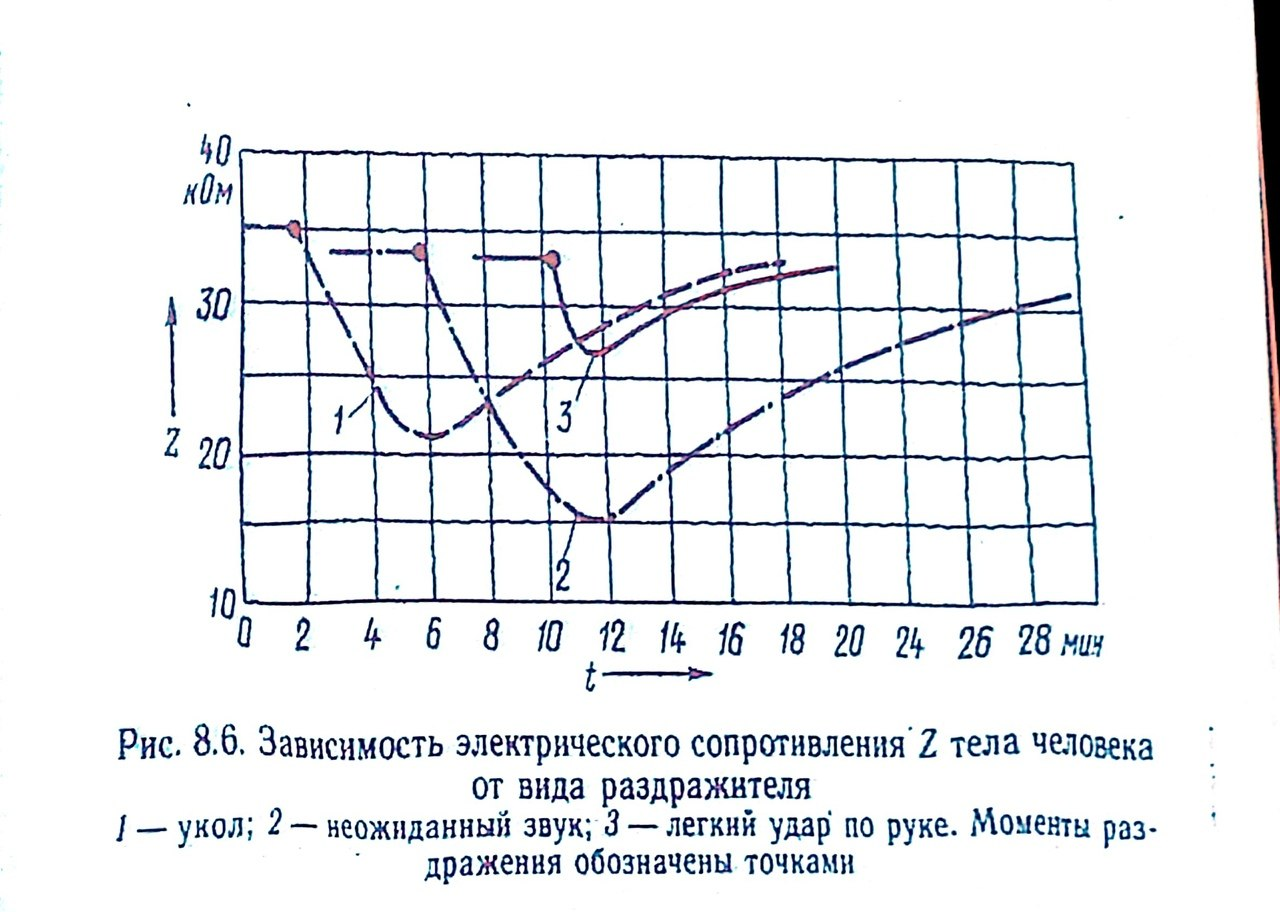
\includegraphics[width=0.8\textwidth]{./img/L2/S002.jpg}
    \caption{График}%
    \label{img:l2:2}
\end{figure}

\begin{figure}[h]
    \centering
    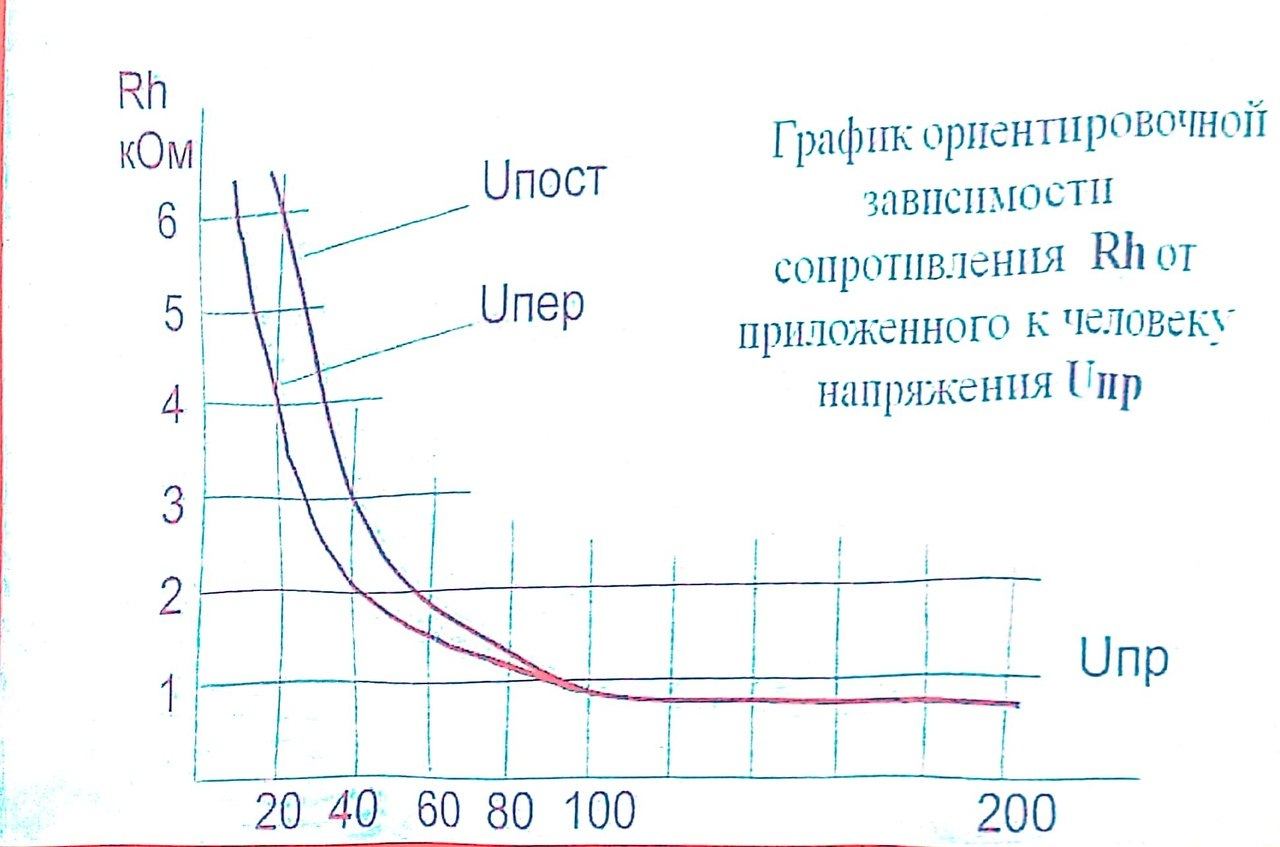
\includegraphics[width=0.8\textwidth]{./img/L2/S001fig.jpg}
    \caption{График}%
    \label{img:l2:1}
\end{figure}

\begin{table}[h]
\centering
\begin{tabular}{@{}lcc@{}}
\toprule
Род и частота тока & \multicolumn{2}{l}{Наибольшие допустимые значения в неаварийном режиме} \\ \midrule
                   & $U_пр$, В                          & $I_i$, мА                          \\ \midrule
Переменный, 50 Гц  & 2                                  & 0.3                                \\
Переменный, 400ГЦ  & 3                                  & 0.4                                \\
Постоянный         & 8                                  & 0.8                                \\ \bottomrule
\end{tabular}
\end{table}

\FloatBarrier{}
\subsection{Прикосновение к токоведущим частям}
\dfn{Двухфазное прикосновение} связано с контактом токоведущих частей двумя конечностями.

\dfn{Однофазное прикосновение} --- контакт одной конечностью.

\begin{itemize}
    \item \dfn{Прямой контакт} --- непосредственное прикосновение к токоведущим частям. Возникает сравнительно редко
    \item \dfn{Косвенный} --- человек трогает металлический корпус электроприбора и т.п., на котором есть опасное напряжение. 
\end{itemize}

С точки зрения последствий оба контакта идентичны.

Электрические параметры, характеризующие связь сети с землей:
\begin{itemize}
    \item Сопротивление изоляции
    \item Емкость относительно земли
    \item Заземления
\end{itemize}
\subsubsection*{Сопротвление изоляции}
$R_u$ --- показатель способности изоляционных конструкций пропускать электрический ток под действием приложенного к этим конструкциям постоянного напряжения
\begin{equation}
r_\phi = {\left( \sum\limits^{n}_{i=1} \dfrac{1}{R_{\phi i}} \right)}^{-1}
\end{equation}
\begin{equation}
    R_{\text{н.экв}} = {\left( \sum\limits_{\phi = A,B,C } \dfrac{1}{r_\phi} \right)}^{-1}
\end{equation}

\subsubsection*{Емкость относительно земли}

\begin{figure}[h]
    \centering
    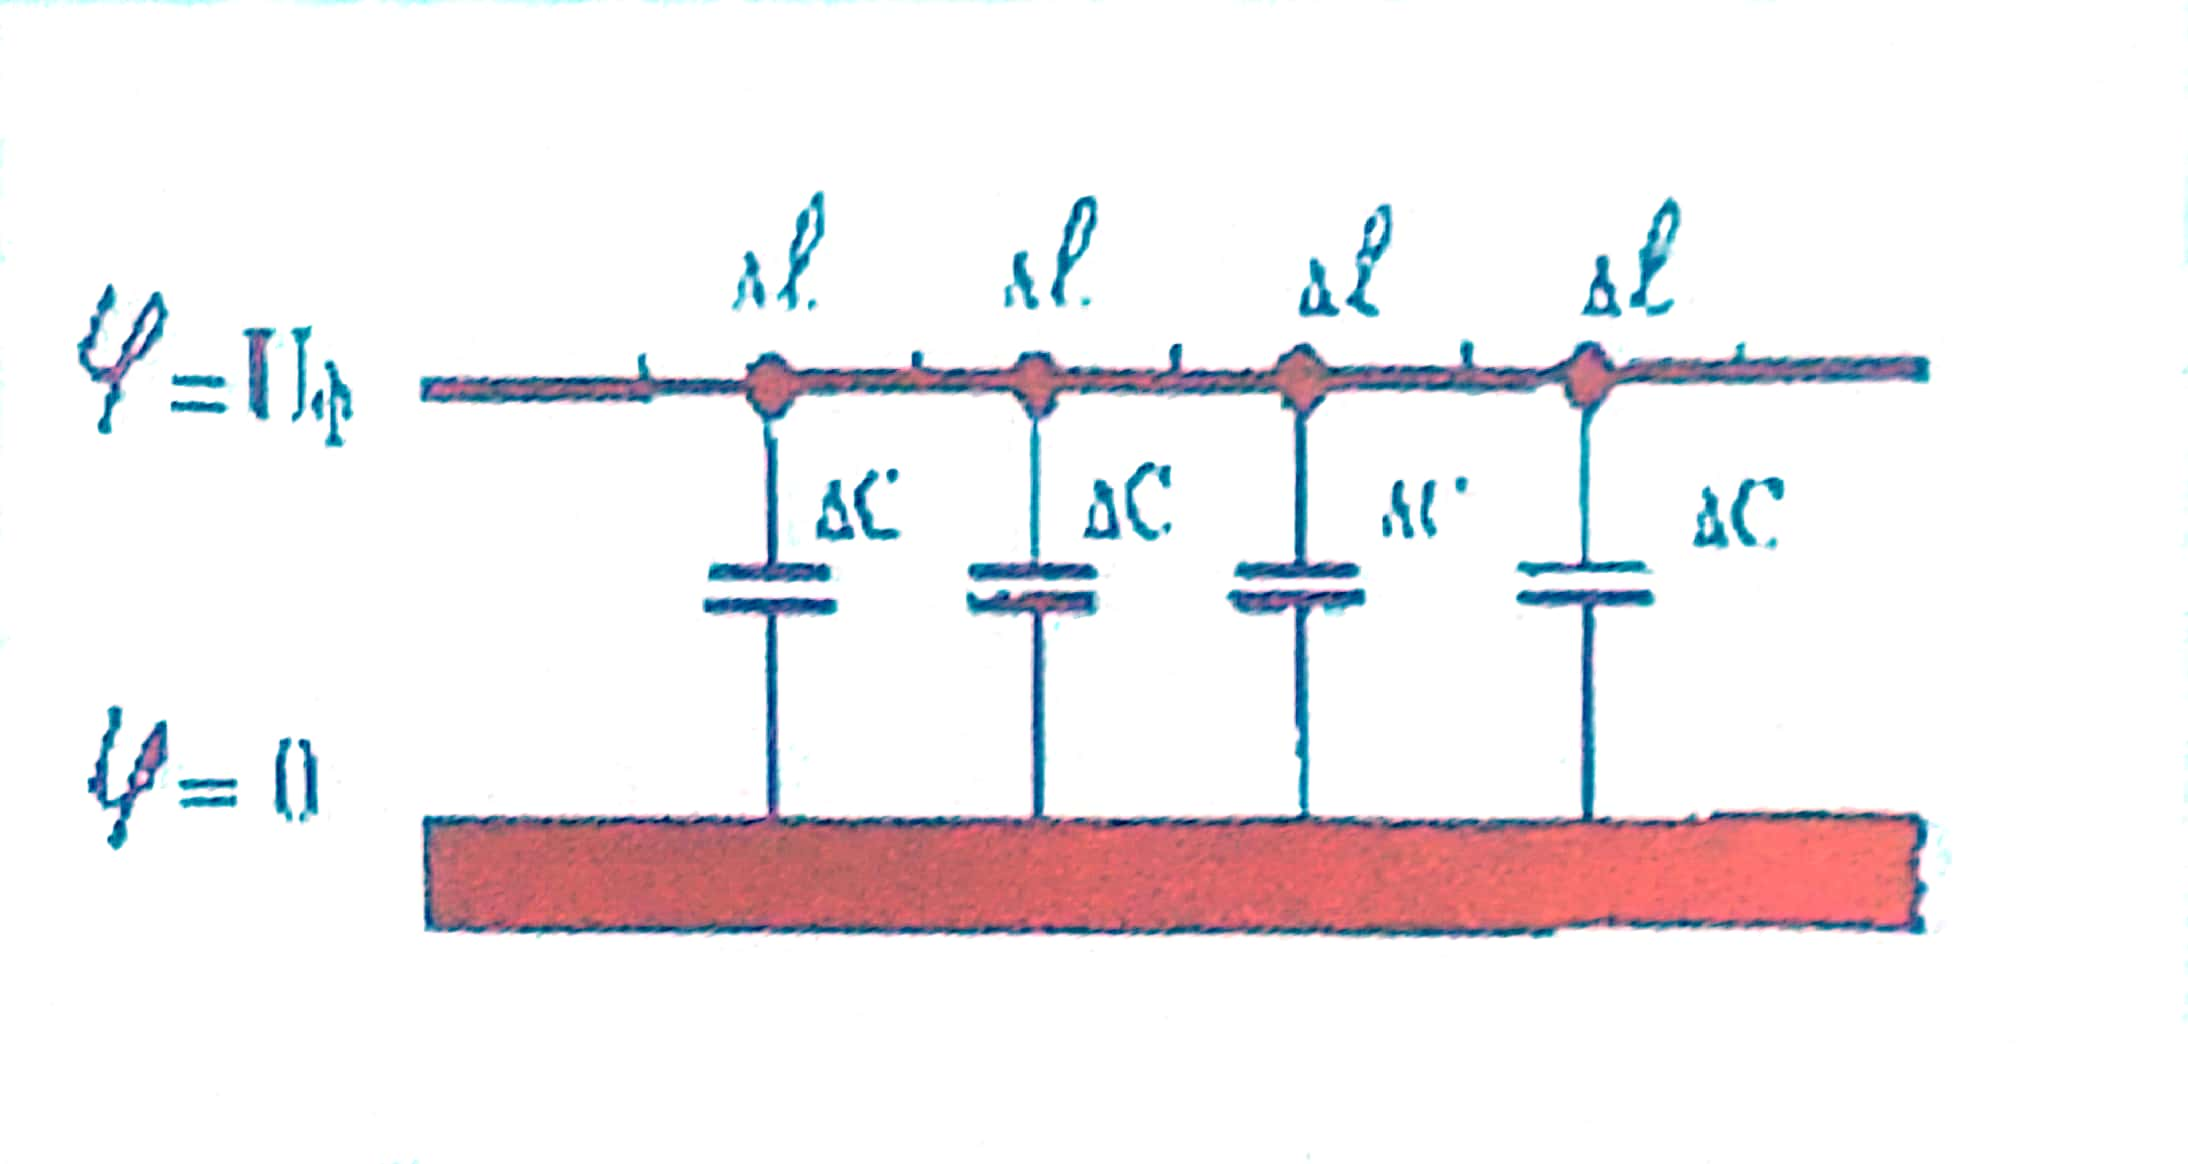
\includegraphics[width=0.7\textwidth]{./img/L2/S003.jpg}
    \caption{Картинка}%
    \label{img:l2:3}
\end{figure}

\begin{equation}
    x_C = \frac{1}{\omega C} = \frac{1}{2\pi f C}  
\end{equation}

\subsubsection*{Заземление}
\dfn{Заземление} --- намеренное соедиенение металлических токоведующих или нетоковедущих частей с землёй.
\begin{itemize}
    \item Заземление нейтрали источника электроэнергии (рабочее заземление)
    \item Защита от поражения током (защитное заземление)
    \item Защита от радиопомех
\end{itemize}

\begin{table}[h]
\centering
\begin{tabular}{@{}ll@{}}
\toprule
Рабочее напряжение & R\_з, Ом \\ \midrule
127220             & 8        \\
220380             & 4        \\
380660             & 2       \\
\bottomrule
\end{tabular}
\end{table}

\section{Однофазное прикосновение}
Ток через тело человека существенно зависит от утечек в изоляционных конструкциях.
\begin{figure}[h]
    \centering
    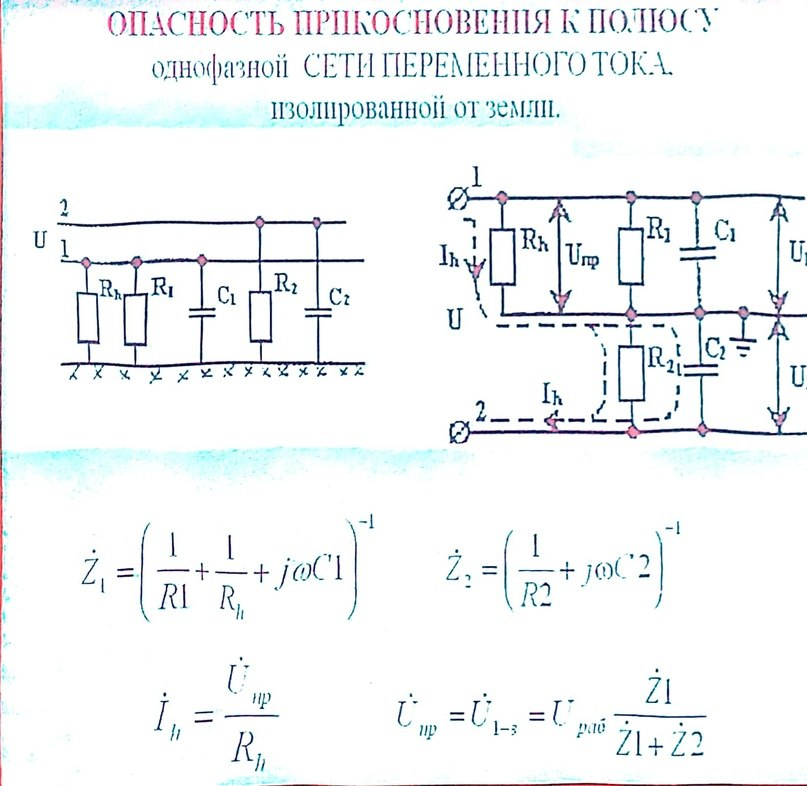
\includegraphics[width=0.95\textwidth]{./img/L3/S001.jpg}
\end{figure}


\begin{figure}[h]
    \centering
    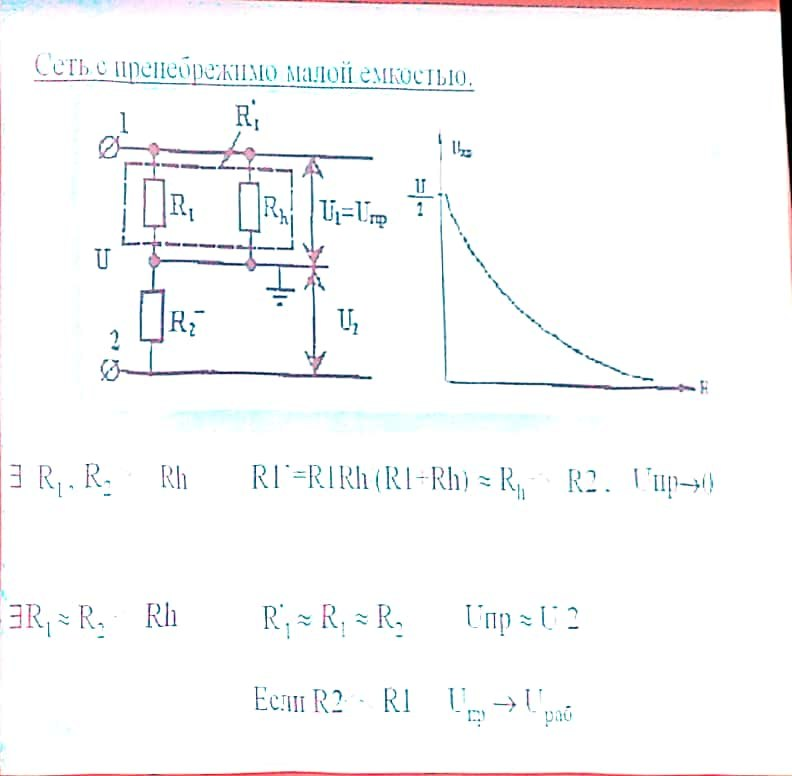
\includegraphics[width=0.95\textwidth]{./img/L3/S002.jpg}
\end{figure}

Условия безопасности прикосновения к токоведущим частям обеспечиваются только в сетях с малой разветвлённостью.

\subsection{Напряжение шага}
Первопричина --- приближение человека к месту замыкания токоведущих частей на землю.

Напряжение шага --- разность потенциалов двух точек поверхности земли, на  которых находится человек

\section{Защитные мероприятия}

\subsubsection*{Организационные защитные мероприятия от поражения электрическим током}

\begin{itemize}
    \item Обучение
    \item Аттестация
    \item Инструктаж
    \item Проверка
\end{itemize}

\subsection{Технические защитные мероприятия}
\begin{itemize}
    \item Исключения (уменьшения вероятности) прикосновения к токоведующим частям вообще или только к находящимся под рабочим напряжением
    \item Исключение возможности (уменьшение вероятности) выноса напряжения сети на нетоковедущие части
    \item Уменьшение величины напряжения прикосновения
    \item Уменьшение длительности протекания через тело человека опасного по величине тока
\end{itemize}

Выбор вида технических средств защиты завиит от:
\begin{itemize}
    \item Степени опасности поражения электрическим током, определяемой
    \begin{itemize}
        \item Параметры электрической сети (рабочее напряжение, уровни сопротивления изоляции и емкости относительно земли, режим нейтрали)
        \item Уровнем квалификации персонала
        \item Условиями размещения оборудования
    \end{itemize}
    \item Требований к обеспечению непрерывности питания электроприемников
    \item Экономических соображений
\end{itemize}

Квалификация персонала:
\begin{itemize}
    \item Электротехнический персонал
    \item Производственный персонал
    \item Население
\end{itemize}

Категории помещений по степени опасности поражения электрическим током:
\begin{itemize}
    \item Без повышенной опасности
    \item С повышенной опасностью
    \item Особо опасные
\end{itemize}

\end{document}
